\begin{enumerate}[label=\thesection.\arabic*.,ref=\thesection.\theenumi]
\numberwithin{equation}{enumi}
\item The root locus of the feedback control system having the characteristic equation $ s^2 + 6Ks + 2s + 5 = 0 $ where
K$>$0, enters into the real axis at
\bigbreak
(A) s = -1
\bigbreak
(B) s = -$\sqrt{5}$
\bigbreak
(C) s = -5
\bigbreak
(D) s = $\sqrt{5}$


\solution

\item Root Locus:
	  Root Locus is a method for plotting the locus of the poles of transfer function for different values of gain parameter K of the function from 0 to $\infty$.

\item How to draw a Root Locus	\\
     Let there be a Open-loop transfer function  $KG(s)$  with unit gain negative feedback. Then the closed-loop transfer function for that particular system is:
    \begin{align}
         \frac{N^{'}(s)}{D^{'}(s)}=\frac{K G(s)}{1+K G(s) H(s)}    
    \end{align}
    
     Then the characteristic equation which gives poles is: 
    \begin{align}
        1+KG(s)H(s)=0
    \end{align}
    
     The locus is symmetric about real axis since all poles are symmetric with real axis.
     
    There are n branches of the locus, one for each Open loop transfer function pole. A Root-Locus line starts at every pole. The locus starts (when $K = 0$) at poles of the open-loop transfer function, and ends (when $K = \infty$) at the zeros.
    
    
    \begin{align}
        K=-\frac{1}{G(s)}=-\frac{D(s)}{N(s)}    
    \end{align}

\item Breakaway Point \\
    While varying 'K', the point where the Root Locus enters real axis is called a 'Breakaway Point'. \\
A breakaway point is the point on a real axis segment of the root locus between two real poles where the two real closed-loop poles meet and diverge to become complex conjugates. Since a Breakaway point corresponds to the point where root locus meets real axis. As the root locus is symmetric about real axis there will be two roots at the Breakaway point. 
i.e.,
    \begin{align}
        \frac{d K}{d s}=-\frac{d}{d K}\left(\frac{D(s)}{N(s)}\right)=0 
    \end{align}
    Once a pole breaks away from the real axis, they can either travel out towards infinity (to meet an implicit zero), or they can travel to meet an explicit zero, or they can re-join the real-axis to meet a zero that is located on the real-axis. 

\item Calculation of Breakaway point \\

Given,the characteristic equation:
    \begin{align}
        s^2 + 6Ks + 2s + 5 = 0    
    \end{align}
    
    Dividing with $s^2 + 2s + 5$ on both sides, we get
    \begin{align}
        1+\frac{6 k s}{s^{2}+2 s+5}=0    
    \end{align}
    This is of form $1+KG(s)=0$ which is closed loop characteristic equation, so that along the root locus
    segments on the real axis ($s = \sigma$)
    \begin{align}
        K=-\frac{1}{G(s)}=-\frac{D(s)}{N(s)}    
    \end{align}

    \begin{align}
        \frac{d K}{d s}=-\frac{d}{d K}\left(\frac{D(s)}{N(s)}\right)=0    
    \end{align}
    \begin{align}
        K=\frac{-\left(s^{2}+2 s+5\right)}{6 s}=-\frac{1}{6}\left[s+2+\frac{5}{s}\right]    
    \end{align}
    And,
    \begin{align}
        \frac{d k}{d s}=0 \Rightarrow\left[1-\frac{5}{s^{2}}\right]=0 
    \end{align}
    Solving for s, we get
    \begin{align}
        s^{2}-5=0 \Rightarrow s=\pm \sqrt{5}    
    \end{align}
    Since, 's' can only be in left half of plane
    \begin{align}
        \boxed{s=-\sqrt{5}}    
    \end{align}
    
    Therefore the Breakaway point is at ($-\sqrt{5}$,0)

    
\item Root Locus plot

	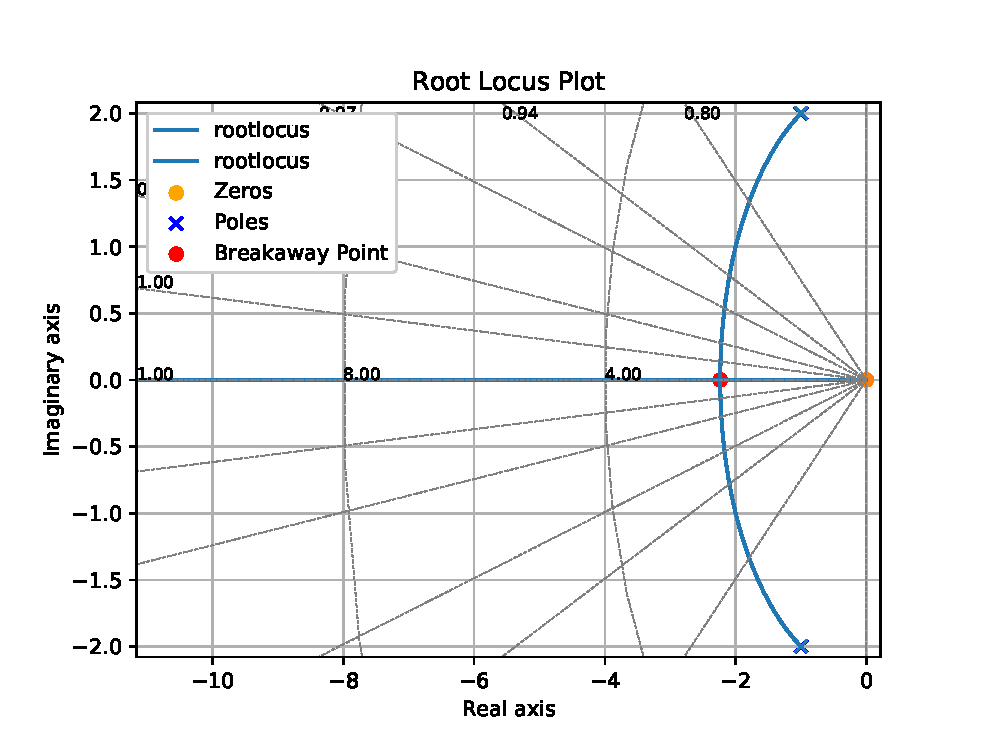
\includegraphics[width=\columnwidth]{./figs/ee18btech11046.eps}

\begin{lstlisting}
codes/ee18btech11046.py
\end{lstlisting}    

\end{enumerate}

